\documentclass[11pt,a4paper,english,oneside, pdf]{article}
\usepackage[margin=2.5cm]{geometry}
\usepackage[utf8]{inputenc} %Permite introducir directamente acentos: á en lugar de \'a etc.
\usepackage{mathtools}
\usepackage{palatino}
\usepackage{graphicx}
\usepackage{hyperref}
\usepackage{xcolor}
\usepackage{tikz}
\usetikzlibrary{shapes.geometric, arrows}


\title{BACoN analysis RUN 3}
\author{Carmen Romo Luque}

\graphicspath{{/Users/romoluque_c/Repositories/BACON_romo/analysis_documentation_run3/images/}}

\begin{document}
	\maketitle
	
	
	\tableofcontents
	
	
	\clearpage
	
	\section{Introduction}	 
	 The BACoN detector is designed to investigate the scintillation properties of liquid argon when doped with xenon. The setup consists of a 100-liter cylindrical cryostat filled with liquid argon, featuring a single upward-facing PMT mounted at the bottom and four rows of three equidistantly spaced SiPMs. Each SiPM row is separated by 10 cm from the next one. On top of the cylinder, an Americium source is placed, emitting gammas and alphas that interact with the liquid, producing scintillation light. The first row of SiPMs is positioned close to the decay source and serves as the trigger system when all of them detect at least one photoelectron. These three SiPMs are collimated to prevent potential saturation effects.
	 
	 %\begin{figure}[!h]
	 %	\begin{center}
	 %		\includegraphics[width=9cm]{BACoN_picture_run2}
	 %		\caption{New setup of the BACoN detector. The PMT is placed at the bottom of the chamber and 4 rows of SiPMs arranged around 10 cm apart, facing the americium source.}
	 %		\label{fig:BACoN_picture_run2}
	 %	\end{center}
	 %\end{figure}
	 
	 The cryostat's liquid argon level is continuously monitored by measuring its weight. Additionally, the argon undergoes purification via a SAES PS4-MT3/15-R getter, which removes impurities such as H$_2$0, CO, CO$_2$, N$_2$, H$_2$, CH$_4$, reducing their concentrations to less than 1 part per billion (PPB) prior to liquefaction.
	 
	 
	 \clearpage
	 
	 \section{Nomenclature}
	 
	 \begin{itemize}
	 	\item \textbf{Channel:}  individual readout or signal processing pathway associated with a single detector. In BACoN each detector (SiPM or PMT) corresponds to a channel. In LEGEND-200 for example, 9 SiPMs make one channel.
	 	\begin{itemize}
	 		\item Channels 0-8: non-trigger SiPMs.
	 		\item Channels 9-11: trigger/source SiPMs.
	 		\item Channel 12: PMT.
	 	\end{itemize}
	 	
	 	\item \textbf{Waveform:} time-dependent electrical signal produced by the detector in response to photon interactions.
	 	
	 	\item \textbf{Event:} coincident set of signals corresponding to a physical interaction that occurs within a defined time window, recorded across multiple SiPM and PMT channels. Each event comprises the waveforms from all SiPM and PMT channels that capture the interaction, allowing the reconstruction of the event's spatial, temporal, and energy characteristics.
	 	
	 	\item \textbf{Run:} continuous set of data that start the same day and are collected over a single or subsequent days (in the case of BACoN), including multiple files that sequentially store the recorded information. No hardware changes are introduced within a run.
	 	
	 	\item \textbf{Period:} set of subsequent runs with the same hardware conditions. For example a new period should start when adding a different amount of xenon doping.
	 	
	 	\item \textbf{Hit:} represents the timestamp (or sample number), energy (in ADC or PE) and channel of each individual peak of photons.
	 \end{itemize}
	  
	 
	
	\clearpage
	
	\section{Data analysis flow}
	\label{data_analysis_flow_sec}
	
	Diagram with the analysis steps:
	
	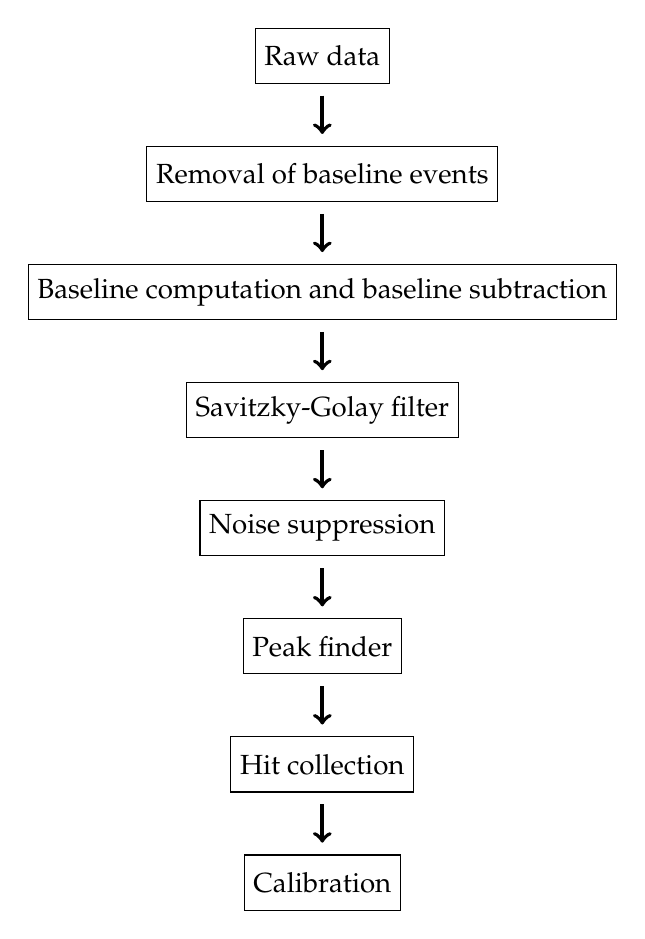
\begin{tikzpicture}[node distance=1.5cm]
		% Define styles for the blocks and arrows
		\tikzstyle{block} = [rectangle, draw, text centered, minimum height=0.7cm]
		%\tikzstyle{arrow} = [thick,->,>=stealth]
		\tikzstyle{arrow} = [thick,->,>=to, shorten >=1.5mm, shorten <=1.5mm, line width=0.5mm]
		
		
		% Define the nodes (blocks)
		\node (raw) [block] {Raw data};
		\node (removal) [block, below of=raw] {Removal of baseline events};
		\node (computation) [block, below of=removal] {Baseline computation and baseline subtraction};
		\node (filter) [block, below of=computation] {Savitzky-Golay filter};
		\node (noise) [block, below of=filter] {Noise suppression};
		\node (peakf) [block, below of=noise] {Peak finder};
		\node (hits) [block, below of=peakf] {Hit collection};
		\node (calibration) [block, below of=hits] {Calibration};

		% Draw arrows between the blocks
		\draw [arrow] (raw) -- (removal);
		\draw [arrow] (removal) -- (computation);
		\draw [arrow] (computation) -- (filter);
		\draw [arrow] (filter) -- (noise);
		\draw [arrow] (noise) -- (peakf);
		\draw [arrow] (peakf) -- (hits);
		\draw [arrow] (hits) -- (calibration);
	\end{tikzpicture}
	
	\subsection{Raw data}
	\label{raw_data_sec}
	
	In BACoN, a new event begins when the three trigger SiPMs detect at least one photoelectron each. Once this condition is met, data from all the sensors are recorded. The raw data are saved in ROOT files. Figure \ref{fig:rawdata} shows an example of the individual signals for an event: the top panel shows signals from all the SiPMs (ordered according to their geometrical location, with channels 9, 10 and 11 being the trigger SiPMs), and the bottom panel shows the signal from the PMT (channel 12). In each event, the three trigger SiPMs always register signal (which triggers the event), while most of the other channels do not detect light. Occasionally, one or more channels will show peaks corresponding to gamma interactions in the liquid argon. For example, the plot for channel 8 shows a single-photon peak. The signal of the trigger SiPMs is inverted due to the amplifier, since the discriminator for the trigger system only accepts negative signals.
	
		\begin{figure}[!h]
			\begin{center}
				\includegraphics[width=\textwidth]{rawdata_sipms.pdf}
				
				\vspace{0.6cm}
				\includegraphics[width=0.5\textwidth]{rawdata_pmt.pdf}
				\caption{Example of an event recorded in BACoN. The three plots in the first row correspond to the trigger SiPMs, which always register signal, as this is the condition for an event to begin. The nine plots in the following rows show signals from the non-trigger SiPMs: channels 0, 1, and 2 are in the bottom row; channels 3, 4, and 5 are in the middle row; and channels 6, 7, and 8 are in the top row, closer to the trigger SiPMs. The distance between rows is approximately 15 cm. The plot at the bottom shows the PMT (channel 12) signal, which is also inverted, as is the case for the trigger SiPMs.}
				\label{fig:rawdata}
			\end{center}
		\end{figure}
		
	
	\subsection{Baseline}
	\label{baseline_sec}
	
	
	The first check of the SiPMs and the PMT data is the baseline. The baseline is computed event by event and channel by channel. It can be computed using either the mean or the mode of the entire waveform, or by selecting a specific range. Since the trigger time in BACoN is close to 1500 ns, we use the first 1300 ns of the waveform to avoid including peaks in the selected region, as shown in blue in Figure \ref{fig:baseline_region}. The distributions using the mode and the mean can be seen in Figure \ref{fig:baselines2} and Figure \ref{fig:baselines3} for the non-trigger channels and the trigger channels, respectively. In the plots we can see that the distribution is narrower when using the mean.
	
	\begin{figure}[!h]
		\begin{center}
			\includegraphics[width=0.8\textwidth]{Baseline_region.pdf}
			\caption{Multiple waveforms from a trigger SiPM showing the trigger time. The region before the trigger time, shown in blue, is used to compute the baseline in order to minimize the influence of any peaks that could interfere with the baseline calculation.}
			\label{fig:baseline_region}
		\end{center}
	\end{figure}
	
	\begin{figure}[!h]
		\begin{center}
			\includegraphics[width=\textwidth]{baselines_rel1_pretrigg.pdf}
			\caption{Relative baseline (baseline - mean of the baseline) for the non-trigger SiPMs using the mode (left) and the mean (right).}
			\label{fig:baselines2}
		\end{center}
	\end{figure}
	
	\begin{figure}[!h]
		\begin{center}
			\includegraphics[width=\textwidth]{baselines_rel1_trigg_pretrigg.pdf}
			\caption{Relative baseline (baseline - mean of the baseline) for the trigger SiPMs using the mode (left) and the mean (right).}
			\label{fig:baselines3}
		\end{center}
	\end{figure}
	
	Figure \ref{fig:baselines_rel1_ch0_whole_and_pretrigg} shows the cases of the mode (left) and the mean (right) for one channel comparing the use of the whole waveform in blue and the region before the trigger time in orange. The distribution using the mode is narrower for the two cases compared to the mean, although it is cleaner and there are no subsequent peaks.
	
	\begin{figure}[!h]
		\begin{center}
			\includegraphics[width=\textwidth]{baselines_rel1_ch0_whole_and_pretrigg.pdf}
			\caption{Comparison of the baseline for one SiPM channel, using the mode (left) and the mean(right) for the whole waveform (blue) comparing with the region before the trigger time (orange).}
			\label{fig:baselines_rel1_ch0_whole_and_pretrigg}
		\end{center}
	\end{figure}
	
	Figure \ref{fig:baselines} shows the baseline over time for the whole data taking period. The baseline has been computed using the mean (solid line) and the mode (dashed line) of the pre-trigger region. The baseline appears to decrease over time, and the deviation from the mean is larger in the trigger SiPMs compared to the regular SiPMs.
	
	\begin{figure}[!h]
		\begin{center}
			\includegraphics[width=0.48\textwidth]{baselines_rel_all_runs.pdf}
			\includegraphics[width=0.48\textwidth]{baselines_rel_all_runs_trigg_chs.pdf}
			\caption{Relative baseline over time using the mean (solid lines) and the mode (dashed lines) of the pretrigger region for the non-trigger SiPMs (left) and for the trigger SiPMs (right).}
			\label{fig:baselines}
			\end{center}
	\end{figure}
	
	%\setlength{\parskip}{10pt}
	\vspace{1cm}

	Another way to compute the baseline (and the one we will use from now on) is by averaging the waveform counts before the trigger region, while rejecting those above a certain threshold. Figure \ref{fig:baseline_computation_final} shows, in black, a waveform from a trigger SiPM with the negative peak corresponding to the trigger time, and in blue, the waveform of a non-trigger SiPM. The pretrigger region is shadowed in grey. In the signal in blue, a peak from a background interaction appears within the pre-trigger region and can affect the baseline computation. To reject this peak, we consider only the waveform counts that fall within 3 standard deviations of the waveform's mean for that particular channel (see waveform in orange).
	
	\begin{figure}[!h]
		\begin{center}
			\includegraphics[width=0.7\textwidth]{baseline_computation_final.pdf}
			\caption{Waveforms from a trigger SiPM (black) and a non-trigger SiPM (blue). The grey region corresponds to the pre-trigger interval, which always precedes the trigger time, indicated by the negative peak in the black waveform. The orange segment highlights the portion of the non-trigger waveform used for baseline computation, excluding signals from background events. This selection was made by applying a threshold of 3 times the standard deviation of the waveform.}
			\label{fig:baseline_computation_final}
		\end{center}
	\end{figure}
	
	The same procedure is applied to the trigger SiPMs (see Figure \ref{fig:baseline_computation_final_ch9} for an example from one of the trigger channels). The baseline exhibits higher noise compared to the non-trigger channels due to the different preamplifier used. Furthermore, as shown in Figure \ref{fig:baseline_example_trigg_chs}, the baseline noise varies among the three trigger SiPMs. For illustrative purposes, the baselines have been plotted sequentially.
	
	\begin{figure}[!h]
		\begin{center}
			\includegraphics[width=0.7\textwidth]{baseline_computation_final_ch9.pdf}
			\caption{Baseline computation for one of the trigger channels.}
			\label{fig:baseline_computation_final_ch9}
		\end{center}
	\end{figure}
	
	\begin{figure}[!h]
		\begin{center}
			\includegraphics[width=0.7\textwidth]{baseline_example_trigg_chs.pdf}
			\caption{Baselines for the three trigger SiPMs, plotted sequentially for illustrative purposes.}
			\label{fig:baseline_example_trigg_chs}
		\end{center}
	\end{figure}
	
	
	
	
	
	The resulting baselines using the mode (left) and the mean (right) are illustrated in Figure \ref{fig:baselines_rel1_ch0_whole_and_pretrigg_new_bsl}. In the case of the mode, the baseline computation remains unaffected—the distribution maintains a similar width—since any peaks that may occasionally fall within the region are not the most frequent values and therefore do not influence the mode. In contrast, when using the mean, the secondary peaks of the disappear, resulting in a much cleaner baseline distribution.
	
	\begin{figure}[!h]
		\begin{center}
			\includegraphics[width=\textwidth]{baselines_rel1_ch0_whole_and_pretrigg_new_bsl.pdf}
			\caption{Comparison of the baseline for one SiPM channel using the mode (left) and the mean (right). Each case shows the baseline computed using the pre-trigger region without any threshold (blue) and with a 3-standard-deviation threshold (orange).}
			\label{fig:baselines_rel1_ch0_whole_and_pretrigg_new_bsl}
		\end{center}
	\end{figure}
	
	
	
	\subsubsection{Baseline at beginning and end of waveform}
	
	We can also compare the baseline, using our chosen method, at the beginning and end of the waveform. In both cases, the results are nearly identical, with the two 2D distributions appearing almost symmetric, as shown in Figure \ref{fig:baselines_init_final_wf_2d_ch0}. The mode case (left) exhibits a more spherical distribution, while the mean case (right) features a narrower core with a broader spread, caused by a few events in the right tail. From these results, we conclude that computing the baseline using a range at either the beginning or the end of the waveform has no significant impact on our data analysis.
	
	\begin{figure}[!h]
		\begin{center}
			\includegraphics[width=0.8\textwidth]{baselines_init_final_wf_2d_ch0.pdf}
			\caption{2D histograms of the baseline values obtained at the beginning and end of the waveforms using the mode (left) and the mean (right).}
			\label{fig:baselines_init_final_wf_2d_ch0}
		\end{center}
	\end{figure}
	
	
	\subsubsection{Baseline subtraction}
	
	After computing the baseline of each individual waveform, it must be subtracted to accurately quantify the amount of light in the signal. This quantification can be performed either by measuring the peak height or by calculating the integral. Figure \ref{fig:bsl_subt_wf} shows an example of an original waveform with a single peak at the center of the window (left), and the same waveform after baseline subtraction (right). The waveform is centered at 0 after baseline subtraction.
	
	\begin{figure}[!h]
		\begin{center}
			\includegraphics[width=\textwidth]{Baseline_subtraction_wf.pdf}
			\caption{Left: Original waveform from a single channel. Right: Same waveform after baseline subtraction.}
			\label{fig:bsl_subt_wf}
		\end{center}
	\end{figure}
	
	\subsection{Convolution and baseline subtraction for trigger SiPMs}
	\label{conv_and_bsl_subt_sec}
	
	In the case of the trigger SiPMs, the signal is inverted by the amplifier because the discriminator processes negative signals. Therefore, before computing and subtracting the baseline, we need to deconvolve the waveforms. Figure \ref{fig:Trigger_SiPM_conv_wf} shows the waveform of a trigger channel before (left) and after (right) deconvolution and baseline subtraction.

	\begin{figure}[!h]
		\begin{center}
			\includegraphics[width=\textwidth]{Trigger_SiPM_conv_wf.pdf}
			\caption{Left: Original waveform from a trigger channel. Right: Same waveform after convolution and baseline subtraction.}
			\label{fig:Trigger_SiPM_conv_wf}
		\end{center}
	\end{figure}
	
	
	\clearpage
	
	\subsection{Savitzky-Golay filter}
	\label{sg_filter_sec}
	
	The goal of the BACoN analysis is to determine the time and amplitude of the signal peaks detected by our sensors. Once the waveforms are centered at zero, it is necessary to apply a threshold to reject noise. However, noise fluctuations can be mistaken for signal if they exceed the selected threshold. To mitigate this issue, we employ the Savitzky-Golay (SG) filter, which effectively removes noise from signals while preserving important features such as peaks and valleys. It is particularly useful when analyzing noisy data, as it enables a clearer interpretation of the underlying signal.
	
	The waveform if smooth in a process known as convolution, by fitting successive sub-sets of adjacent data points with a low-degree polynomial (the degree can be chosen by the user) by the method of linear least squares. A fixed-size window (number of points) is slid across the data. Then, within each window, a polynomial is fitted to the data. The function that we use in Python is \texttt{scipy.signal.savgol\_filter} and parameters are \texttt{window\_length=30} and  \texttt{polyorder=3}.
	
	\begin{figure}[!h]
		\begin{center}
			\includegraphics[width=9cm]{SG_filter_wf_close.pdf}
			\caption{Subtracted waveform (blue) and the same waveform (black) after applying the Savitzky-Golay filter.}
			\label{fig:SG_waveform}
		\end{center}
	\end{figure}
	
	Figure \ref{fig:SG_waveform} shows a subtracted waveform and the result after filtering applying the Savitzky-Golay filter. As depicted in Figure \ref{fig:SG_waveform_thr}, this filter ensures that no baseline fluctuations exceed the desired threshold.
	
	\begin{figure}[!h]
		\begin{center}
			\includegraphics[width=\textwidth]{SG_waveform_wl30ns_thr_points.pdf}
			\caption{Left: subtracted waveform. Right: subtracted and filtered waveform. The points above the chosen threshold (e.g., 30 ADC) are shown to illustrate that, after filtering, no baseline noise exceeds the threshold, reducing the risk of misinterpreting noise as signal.}
			\label{fig:SG_waveform_thr}
		\end{center}
	\end{figure}
	
	One important consideration when employing this method is that the heights of the peaks may be slightly reduced after filtering. To account for this effect, SiPM calibration should also be performed using the same filtering process.
	
	\subsubsection{Comparison between SG and Wiener filter}
	
	In addition to the SG filter, other signal processing techniques can be employed for noise reduction. One such method is the Wiener filter, which reduces noise by minimizing the mean square error between the estimated and true signals. It adjusts the amount of smoothing based on the local signal-to-noise ratio—that is, how much noise is present in different parts of the signal—while preserving important features. In Python, this filter is available as \texttt{scipy.signal.wiener}, where we used the parameter \texttt{mysize=30}.
	
	Figure \ref{fig:single_pe_shape_ch8_SG_and_Wiener_filter} shows a subtracted waveform in blue, with the results of applying the SG and Wiener filters shown in black and orange, respectively. The SG filter typically produces a smoother output that follows the general trend of the data. While it may miss sharp transitions, those are not essential for BACoN.
	
	\begin{figure}[!h]
		\begin{center}
			\includegraphics[width=9cm]{single_pe_shape_ch8_SG_and_Wiener_filter.pdf}
			\caption{Subtracted waveform (blue) and the same waveform after applying the Savitzky-Golay filter (black) and the Wiener filter (orange).}
			\label{fig:single_pe_shape_ch8_SG_and_Wiener_filter}
		\end{center}
	\end{figure}
	
	\clearpage
	
	\subsection{Noise suppression}
	\label{noise_suppression_sec}
	
	After filtering the waveforms, it is both useful and computationally efficient to perform zero-suppression. In this method, any values below a certain threshold—used to eliminate noise—are set to zero. This makes peak detection easier for our algorithm and prevents unnecessary data from being stored.
	
	\subsubsection{Threshold applied to the SiPMs}
	
	Choosing the threshold carefully is crucial because we don’t want to miss real light peaks, but at the same time, we need to avoid setting it too low, as this could result in noise or fluctuations being mistakenly identified as real peaks. The threshold also depends on the gain of the channels, as this affects the height of the single photoelectron (SPE) peak. For data from period 3, the typical photoelectron peak height ranges from 100 to 150 ADC for a non-trigger SiPM, while it ranges from 500 to 1000 ADC for a trigger SiPM. Figure \ref{fig:1PE_wfs_and_average_sg} shows multiple SPE waveforms after the SG filter, with the averaged waveform in black, for a chosen non-trigger channel (left) and a trigger channel (right).
	
	\begin{figure}[!h]
		\begin{center}
			\includegraphics[width=0.49\textwidth]{1PE_wfs_and_average_sg_ch8.pdf}
			\includegraphics[width=0.49\textwidth]{1PE_wfs_and_average_sg_ch9.pdf}
			\caption{Single photoelectron peaks after applying the Savitzki-Golay filter with the averaged waveform shown in black for a non-trigger channel (left) and for a trigger channel (right).}
			\label{fig:1PE_wfs_and_average_sg}
		\end{center}
	\end{figure}
	
	In the previous analyses, we used a threshold of 50 ADC for all channels. However, the gain of the sensors in this period is higher, especially for the trigger SiPMs, so we had to reconsider this decision. As shown in Figure \ref{fig:SPE_event_diff_thrs}, a threshold of 50 ADC may be too low, as fluctuations that are identified as peaks can affect the subsequent peak finder analysis.
	
	\begin{figure}[!h]
		\begin{center}
			\includegraphics[width=9cm]{SPE_event_diff_thrs.pdf}
			\caption{Example of a single photoelectron peak for a non-trigger channel. The original waveform is shown in blue, the filtered waveform in black, and the zero-suppressed waveform (using a threshold of 50 ADC) in red. The horizontal lines indicate the two thresholds considered: 50 and 80 ADC. The black circle at the tail of the peak highlights a fluctuation that is mistakenly labeled as a peak.}
			\label{fig:SPE_event_diff_thrs}
		\end{center}
	\end{figure}
	
	
	Therefore, the thresholds chosen are 80 ADC for the non-trigger SiPMs and 200 ADC for the trigger SiPMs. An example of a zero suppressed waveform once the threshold is applied, can be seen in Figure \ref{fig:ZS_SPE_event_thr80ADC}.
	
	\begin{figure}[!h]
		\begin{center}
			\includegraphics[width=9cm]{ZS_SPE_event_thr80ADC.pdf}
			\caption{Example of a single photoelectron peak for a non-trigger channel. The original waveform is shown in blue, the filtered waveform in black, and the zero-suppressed waveform, using a threshold of 80 ADC, in red. The zero supressed waveform has all the values below 80 ADC set to zero.}
			\label{fig:ZS_SPE_event_thr80ADC}
		\end{center}
	\end{figure}
	
	
	\clearpage
	
	\subsection{Pile-up events}
	
	Pile-up occurs when multiple photons arrive to a SiPM within a very short time window, resulting in overlapping signals that the detector cannot distinguish as separate events.
	
	In BACoN, we have observed that, occasionally, there are pile-up signals and these are not straight-forward to deconvolve. To understand these types of events, we should first clarify what a single photoelectron signal looks like. The left side of Figure \ref{fig:1PE_signal} shows multiple single PE waveforms for channel 8 in blue, with their average amplitude in black. The shape of the single PE signal follows a Landau distribution, as seen in the fit on the right side of Figure \ref{fig:1PE_signal}.
	
	\begin{figure}[!h]
		\begin{center}
			\includegraphics[width=0.49\textwidth]{images/1PE_wfs_and_average_ch8.pdf}
			\includegraphics[width=0.46\textwidth]{images/averaged_single_PE_wfs_fit_Landau.pdf}
			\caption{Left: superposition of 100 single-photon waveforms for a selected channel (channel 8) in blue, with the averaged waveform in black. Right: fit of the averaged waveform to a Landau distribution.}
			\label{fig:1PE_signal}
		\end{center}
	\end{figure}
	
	The width of the single PE peak depends on the amplitude chosen as the reference. In Figure \ref{fig:width_1PE_signal}, we can see the averaged single PE waveform along with the crossing points at different threshold amplitudes. The red case corresponds to a threshold of 50 ADC, while the green case corresponds to a threshold of 80 ADC.
	
	\begin{figure}[!h]
		\begin{center}
			\includegraphics[width=0.49\textwidth]{images/width_single_PE_peak_ch8.pdf}
			\caption{Single photon averaged waveform with the crossing points at 50 ADC (red) and 80 ADC (green).}
			\label{fig:width_1PE_signal}
		\end{center}
	\end{figure}
	
	The left side of Figure \ref{fig:width_1_and_2_PE} shows the averaged 1PE and 2PE waveforms after smoothing with the Savitzky-Golay filter. The different widths corresponding to the different numbers of photoelectrons can be seen. On the right, the histogram of the widths for multiple waveforms in each case is shown. The mean 1PE widths are 118 ns and 72 ns for threshold values of 50 and 80 ADC, respectively, while the mean 2PE widths are 198 ns and 149 ns for thresholds of 50 and 80 ADC, respectively.
	
	\begin{figure}[!h]
		\begin{center}
			\includegraphics[width=0.49\textwidth]{images/width_1_and_2_PE_peak_sg.pdf}
			\includegraphics[width=0.46\textwidth]{images/width_1_and_2_PE_peak_comparison_hist_norm_ch8.pdf}
			\caption{Left: averaged waveforms for 1 and 2 PEs after filtering with the Savitzky-Golay filter, with the corresponding crossing points at 50 ADC (red) and 80 ADC (green). Right: histogram of the 1 and 2 PE widths for the two different thresholds (50 and 80 ADC) using SG-filtered waveforms from a selected data file.}
			\label{fig:width_1_and_2_PE}
		\end{center}
	\end{figure}
	
	These numbers are crucial for the input parameters in our peak-finding algorithm. In the past, we used a minimum distance between peaks of 30 ns, which is very small compared to the results shown here. The individual events in Figure \ref{fig:pile_up_evts} demonstrate that the minimum distance we should require in our analysis is much greater than 30 ns. The two plots on top correspond to events where no pile-up is present, but instead, fluctuations in the noise. If the wrong minimum distance between peaks and threshold amplitude are chosen, the second peak in the event on the left and the first peak in the event on the right can be incorrectly labeled as valid peaks when they are not. In contrast, the two plots below show pile-up events that we want to keep and attempt to deconvolve to extract their amplitude. These events have a distance between peaks that is always above 100 ns. For these reasons, a threshold of 80 ADC in amplitude was chosen to reject the noise (as shown in Section \ref{noise_suppression_sec}), and a minimum distance of 100 ns between peaks (corresponding to 50 time samples) was set.
	
	\begin{figure}[!h]
		\begin{center}
			\includegraphics[width=0.49\textwidth]{images/pile_up_evt_329_ch8.pdf}
			\includegraphics[width=0.49\textwidth]{images/pile_up_evt_1053_ch8.pdf}
			\includegraphics[width=0.49\textwidth]{images/pile_up_evt_1037_ch8.pdf}
			\includegraphics[width=0.49\textwidth]{images/pile_up_evt_3888_ch8.pdf}
			\caption{The events at the top are examples of low-light events, where fluctuations in the waveform noise can be mislabeled as secondary peaks if the minimum distance between peaks and the amplitude threshold are not properly set. The plots below show pile-up events that we aim to retain, where the secondary peaks correspond to actual photoelectrons detected.}
			\label{fig:pile_up_evts}
		\end{center}
	\end{figure}
	
	
	
	Figure \ref{fig:pile_up} shows an example of a pile-up event that can be recovered, as our algorithm is able to distinguish between the two peaks. However, handling secondary peaks is not straightforward. By overlaying the averaged waveform from Figure \ref{fig:1PE_signal} onto both peaks (black and orange in the right plot), we can see that the first peak corresponds to a single photon, while the second peak is slightly smaller when we align the orange averaged waveform starting from the crossing point with the black averaged waveform.
	
	
	\begin{figure}[!h]
		\begin{center}
			\includegraphics[width=0.49\textwidth]{images/pile_up_evt_8a.pdf}
			\includegraphics[width=0.49\textwidth]{images/pile_up_evt_8.pdf}
			\caption{Left: example of a pile-up event with two clearly separated peaks, which our algorithm can differentiate. Right: the same pile-up event (in blue), with the averaged 1PE waveforms overlaid on the first peak (in black) and the second peak (in orange).}
			\label{fig:pile_up}
		\end{center}
	\end{figure}
	
	
	\clearpage
	
	
	\subsection{Peak finder}
	\label{peak_finder_sec}
	
	\subsubsection{Single PE shape}
	
	\subsubsection{Distance between peaks in non-trigger SiPMs}

	\subsubsection{Distance between peaks in trigger SiPMs}	
	
	\subsubsection{Second peaks analysis method}
	
	\subsubsection{Trigger time}
	
	\subsection{Hit collection and time distribution}
	\label{hits_sec}
	
	
	\subsection{Fit to time distribution of high light events}
	
	\subsubsection{SiPM channels}
	
	During period 3 of data taking, we discovered that the level of liquid argon was just below the radioactive source holder—2 inches lower than expected—which meant that the Americium source and the trigger SiPMs were not submerged in LAr. Before Georgia made this calculation (explained \href{https://www.overleaf.com/project/67e58e00495d6f172b347fb3}{here}), we were unsure of the cause, so we also considered the cleanliness of the LAr as a potential issue. However, Claudio Savarese suggested during the LEGEND CM that if we observe the triplet slope for high-light events (muons), it would indicate that the argon is clean and that the issue is likely related to the source. To verify this, we should fit the time distribution for each SiPM; if it is close to 1600 ns, it would correspond to the triplet.
	
	Figure \ref{fig:Fit_tdist_high_light_events} shows the fit to the time distribution of high-light events for each individual non-trigger SiPM. Channels 1 and 4 are plotted in grey to highlight that they have special foils on their surfaces, which affect their time distributions. For the other channels, the decay constant $\tau$ ranges from 1.3 to 1.7 $\mu$s, values that are close to the expected triplet decay time of 1.6 $\mu$s.
	
	\begin{figure}[!h]
		\begin{center}
			\includegraphics[width=\textwidth]{images/Fit_tdist_high_light_events.pdf}
			\caption{Time distribution obtained using the hits and timestamps from high-light events in BACoN (events above 1000 ADC) for each individual SiPM channel. All channels are shown in blue with their corresponding fit, except for channels 1 and 4, which are shown in grey due to additional foils on their surfaces: a quartz window that blocks 128 nm light for channel 1, and a polycarbonate window that blocks all light below 400 nm for channel 4.}
			\label{fig:Fit_tdist_high_light_events}
		\end{center}
	\end{figure}

	Figure \ref{fig:Fit_tdist_high_light_events_trigg} instead, shows the time distributions fitted for the trigger SiPMs, with values between 1600 and 1800 ns.
	
		\begin{figure}[!h]
		\begin{center}
			\includegraphics[width=\textwidth]{images/Fit_tdist_high_light_events_trigg.pdf}
			\caption{Time distribution obtained using the hits and timestamps from high-light events in BACoN (events above 3000 ADC) for each individual trigger channel. The linear fit with the corresponding decay time is shown in red.}
			\label{fig:Fit_tdist_high_light_events_trigg}
		\end{center}
	\end{figure}
	
	
	\subsubsection{PMT}
	
	We also examined the high-light events in the PMT. As shown in Figure \ref{fig:Fit_tdist_high_light_events_PMT}, the triplet component is only visible for high-light events—those with at least one peak above 1500 ADC in the phototube—corresponding to the blue line. The distribution of non-high-light events is shown in red.
	
	When fitting the time distribution from the high-light events, we obtained a decay constant between 1.5-1.6 $\mu$s, which is significantly higher than in the SiPM case. However, according to the quantum efficiency of our PMT (Hamamatsu model R11410-10), shown in Figure \ref{fig:pmt_QE} as a function of wavelength, and considering the absence of any wavelength-shifting material, the PMT should not be sensitive to argon scintillation light. Therefore, this light is likely due to residual xenon or Cherenkov radiation produced by muons.
	
	\begin{figure}[!h]
		\begin{center}
			\includegraphics[width=12cm]{images/Fit_tdist_high_light_events_PMT.pdf}
			\caption{Time distribution of the events detected by the PMT. The distribution corresponding to high-light events is shown in blue, along with the corresponding triplet fit yielding a decay constant of 2561 ns. The time distribution of the remaining events is shown in red.}
			\label{fig:Fit_tdist_high_light_events_PMT}
		\end{center}
	\end{figure}
	
	\begin{figure}[!h]
		\begin{center}
			\includegraphics[width=12cm]{images/pmt_QE.pdf}
			\caption{Quantum efficiency for the PMT used in BACoN, from Hamamatsu model R11410-10.}
			\label{fig:pmt_QE}
		\end{center}
	\end{figure}
	
	
	\clearpage

	\subsubsection{All channels together}
	
	We can also split the data by month—from September 2024 to January 2025—fit the data, and compute the decay constant for each individual month and each channel. Figure \ref{fig:Fit_tdist_high_light_events_tau_months_with_trigg_chs_and_pmt} displays the decay constant $\tau$ for each channel in a consistent color, where each point of the same color corresponds to one of the five months of data taking. All non-trigger channels (except for 1 and 4 that have special foils covering their surface) have $\tau$ values close to the measured triplet lifetime of 1600 ns. The values obtained for the trigger SiPMs are similar to those of the non-trigger SiPMs, while the PMT values range from 2400 to 2800 ns.
	
	From these results, we can conclude that the distribution we observe comes from the triplet light and the argon is clean enough.
	
	\begin{figure}[!h]
		\begin{center}
			\includegraphics[width=\textwidth]{images/Fit_tdist_high_light_events_tau_months_with_trigg_chs_and_pmt.pdf}
			\caption{Decay constant obtained from the linear fit for each invidiual channel (SiPMs and PMT) and each month of data taking. The grey horizontal dashed line corresponds to the triplet lifetime value at 1600 ns.}
			\label{fig:Fit_tdist_high_light_events_tau_months_with_trigg_chs_and_pmt}
		\end{center}
	\end{figure}
	
	\vspace{1cm}
	
	\begin{figure}[!t]
		\begin{center}
			\includegraphics[width=\textwidth]{images/SF_high_light_evts_all_chs.pdf}
			\caption{Survival fraction of high light events for the non-trigger channels (blue), the trigger channels and the PMT (both in red).}
			\label{fig:SF_high_light_evts_all_chs}
		\end{center}
	\end{figure}
	
	The survival fraction of high-light events for all channels is shown in Figure \ref{fig:SF_high_light_evts_all_chs}. The values for the trigger channels and the PMT are considerably higher—on the order of 10\%—compared to the $\sim$0.1\% observed in the non-trigger channels. These higher values are plotted using the red color and the right y-axis. Channels 0 to 8 exhibit similar survival fractions (with channels 1 and 4 slightly lower, possibly due to their special foils), while among the trigger SiPMs, there is a significant jump between channel 9 and the other two.
	
	
	\clearpage
	
	\subsection{Sum of the 1PE waveforms}
	\label{sum_wfs_sec}
	
	
	
	\subsection{SiPM calibration}
	\label{calibration_sec}
	
	Maintaining the optimal performance of sensors in the BACoN system is crucial for accurate data collection, enabling the detection of variations in light levels within the detector. For this, periodic calibrations of the SiPMs are conducted to verify their proper functioning and stability. Despite employing the same sensor model across all SiPMs, variations in analog-to-digital conversion (ADC) counts in response to identical light inputs are inevitable. Hence, regular calibration of the SiPMs at the single photon level is imperative to standardize their responses and assess their long-term stability.
	
	Ideally, a chamber should be equipped with LEDs for performing regular calibrations during data collection. That would allow us to monitor gain variations over time at a controlled light intensity, particularly important for long-term data acquisitions lasting several months or few years. Additionally, since we operate at low temperatures, the gains of the SiPMs won't match those obtained during black box calibration. However, in the absence of LEDs, we can still utilize low-light data for similar calibrations, though it's important to note that the values may differ.
	
	Due to the low temperature required to maintain argon in its liquid state within the BACoN detector, the bias voltage of the SiPMs needs to be reduced. This compensates for the decrease in breakdown voltage of the silicon diodes within the SiPM structure under reduced thermal conditions. At lower temperatures, the breakdown voltage tends to increase, meaning that the same bias voltage applied at room temperature could potentially cause the SiPMs to operate in a regime where the breakdown voltage is exceeded. This can lead to excess dark count rate and decreased performance. Therefore, reducing the bias voltage when operating SiPMs at lower temperatures helps ensure that they remain within their optimal operating conditions and maintain stable performance. That's the reason why the gains of the SiPMs inside the chamber are higher even at a lower bias voltage.
	
	
	First, we subtract the baseline of the waveform, which allows us to obtain the absolute height of the peaks. The baseline subtraction procedure can be performed by computing either the mean value or the mode of the entire waveform or just a certain range. 
	Then, we compute the single photon spectra by getting the height of the peaks at the trigger region. 
	
	
	Subsequently, a histogram is generated displaying the heights of the peaks in the trigger window, allowing for the identification of individual single photoelectron peaks. First, a poisson distribution of a certain number of gaussians is perfomed in order to extract the mean position of each photoelectron peak. The gain is then calculated from the spectrum using the distance between the pedestal peak and those for 1, 2, ...  photoelectrons.
	
	
	Then, the linear regression of the mean achieved enables the extraction of the conversion factor between ADC and photoelectrons. With these values, the response across all channels can be standardize.
	
	\clearpage
	
	\section{Sum of detected photoelectrons in the trigger channels}
	
	\begin{figure}[!h]
		\begin{center}
			\includegraphics[width=0.58\textwidth]{images/trigger_SiPMs_light_sum.png}
			\hspace{3mm}
			\includegraphics[width=0.38\textwidth]{images/trigger_SiPMs_light_sum_LLAMA.png}
			\caption{Sum of detected photoelectrons (PE) in all three source SiPMs for BACoN (left) and LLAMA (right). In both cases, at low light levels, individual photoelectrons can be distinguished starting at 3 PE, as the trigger condition required that at least one photon be detected by each channel. In the LLAMA plot, the peak is attributed to the full energy deposition of 60 keV gamma particles emitted from the $^{241}$Am source. In BACoN, this peak is absent, which needs further investigation.}
			\label{fig:sum_detected_pe_trigger_chs}
		\end{center}
	\end{figure}
	
	
	
	\clearpage
	\section{PMT analysis}
	
	In BACoN, there is one PMT at the bottom of the chamber, facing upwards. It is primarily sensitive to blue light and has no wavelength shifter on its surface, so, in principle, it should be insensitive to argon scintillation light at 128 nm (and barely sensitive to xenon scintillation light at 175 nm).
	
	\subsection{Baseline computation}
	
	A PMT pulse is shown in the bottom plot of Figure \ref{fig:rawdata}. PMTs typically produce a negative output signal, so each waveform needs to be inverted before performing baseline subtraction. As with SiPMs, the baseline is computed by averaging each individual waveform using the region before the trigger time (from 0 to 1300 ns). To avoid including any pulses that might interfere with the calculation, the standard deviation is computed, resulting in $\pm$ 3.5 ADC. Therefore, we take the region in y of the waveform that is within 3$\sigma \times$ std (see orange part of the waveform in Figure \ref{fig:pmt_baseline_comp} and average it.
	
		\begin{figure}[!h]
		\begin{center}
			\includegraphics[width=0.8\textwidth]{images/pmt_baseline_computation.pdf}
			\caption{Selected waveform from the PMT showing the region used to extract the baseline: the grey region corresponds to the pre-trigger region, while the orange region indicates 3$\sigma$ of the standard deviation of the waveform. The horizontal green and red lines correspond to the mean and the mode, respectively, of the orange region.}
			\label{fig:pmt_baseline_comp}
		\end{center}
	\end{figure}
	
	\subsection{Example of bad events in the PMT}
	
	Figure \ref{fig:pmt_bad_evts} shows two examples of events that we want to exclude from our analysis: a ringing event (left) and a saturating event with afterpulsing (right).
	
	
	\begin{figure}[!h]
		\begin{center}
			\includegraphics[width=0.49\textwidth]{images/pmt_bad_evt_95.pdf}
			\includegraphics[width=0.49\textwidth]{images/pmt_bad_evt_831.pdf}
			\caption{Examples of bad events in the PMT. Left: Ringing event. Right: Saturating event with afterpulsing.}
			\label{fig:pmt_bad_evts}
		\end{center}
	\end{figure}
	
	
	\subsection{Light intensity detected by the PMT vs SiPMs}
	
	In a quick test, we computed the maximum of the PMT waveforms and compare with the same event for the SiPM responses. This way we wanted to understand any possible coincidences, such as saturating events, or common scintillation.
	
	Figure \ref{fig:pmt_and_sipm_max} shows the maximum of the waveforms for the PMT compared to the SiPM channel 0. The image on the left of the first row spans the entire dynamic range of the PMT, while the other three cover the ranges 0 to 100 ADC, 0 to 100 ADC, and 0 to 4000 ADC, respectively. In all four plots, the individual regions corresponding to the baseline, 1 PE, 2 PE, and so on, are clearly distinguishable for the SiPM (as shown by the labels in the first plot). For the PMT, the baseline is also noticeable (see the plot on the right in the first row), but the regions corresponding to individual photoelectrons are harder to distinguish. The region from 150 to 850 ADC is considered to correspond to 1 PE, while the subsequent PE regions are not clearly visible.
	
	\begin{figure}[!h]
		\begin{center}
			\includegraphics[width=0.49\textwidth]{images/pmt_max_vs_SiPM0_max.pdf}
			\includegraphics[width=0.49\textwidth]{images/pmt_max_vs_SiPM0_max_rng_0_100.pdf}
			\includegraphics[width=0.49\textwidth]{images/pmt_max_vs_SiPM0_max_rng_0_1000.pdf}
			\includegraphics[width=0.49\textwidth]{images/pmt_max_vs_SiPM0_max_rng_0_4000.pdf}
			\caption{Comparison of the maximum PMT waveform to the maximum waveform for a selected SiPM channel, using different amplitude ranges for the PMT.}
			\label{fig:pmt_and_sipm_max}
		\end{center}
	\end{figure}
	
	
	Figure \ref{fig:pmt_and_trigger_sipm_max} is the equivalent of Figure \ref{fig:pmt_and_sipm_max} but for one of the trigger SiPMs (channel 9). As in the previous figure, the individual photoelectron regions are clearly distinguishable for the SiPM (up to several PE numbers), while for the PMT, the region for single photoelectrons is more spread out, and higher photon numbers cannot be distinguished.
	
	\begin{figure}[!h]
		\begin{center}
			\includegraphics[width=0.49\textwidth]{images/pmt_max_vs_SiPM9_max.pdf}
			\includegraphics[width=0.49\textwidth]{images/pmt_max_vs_SiPM9_max_rng_0_100.pdf}
			\includegraphics[width=0.49\textwidth]{images/pmt_max_vs_SiPM9_max_rng_0_2000.pdf}
			\includegraphics[width=0.49\textwidth]{images/pmt_max_vs_SiPM9_max_rng_0_4000.pdf}
			\caption{Comparison of the maximum PMT waveform to the maximum waveform for a selected SiPM trigger channel, using different amplitude ranges for the PMT.}
			\label{fig:pmt_and_trigger_sipm_max}
		\end{center}
	\end{figure}
	
	\subsection{Saturating events}
	
	By examining the upper range of the previous plots, we can analyze how many events saturate in the PMT in coincidence with the SiPM channels. Figure \ref{fig:saturating_evts} left shows the maximum amplitude of the selected SiPM (channel 0) and Figure \ref{fig:saturating_evts} right displays the selected trigger SiPM (channel 9) at the upper end of the dynamic range for both PMT and SiPM. The plot for channel 0 shows a single bin at the corner with more than a hundred events, likely from muons. In contrast, the plot on the right, which correlates one of the trigger SiPMs with the PMT amplitude, shows no such bin at the corner with a high number of events. This suggests that our source SiPMs do not trigger when, for example, a muon is detected.
	
	The same result is also shown in Figure \ref{fig:saturating_evts2} as a one-dimensional histogram. Figure \ref{fig:saturating_matrix} further illustrates the correlation between pair of channels. The PMT detects most of the energetic events that cause saturation, and there are no clear correlations between pair of channels. The highest correlation is between channels 4 and 7.
	
	\begin{figure}[!h]
		\begin{center}
			\includegraphics[width=0.49\textwidth]{images/pmt_max_vs_SiPM0_max_saturating_evts.pdf}
			\includegraphics[width=0.49\textwidth]{images/pmt_max_vs_SiPM9_max_saturating_evts.pdf}
			\caption{Comparison of the maximum PMT waveform with the maximum waveforms for a selected non-trigger SiPM (left) and a trigger SiPM (right) at the upper end of the dynamic ranges for both the PMT and SiPMs. The absence of events in the corner of the trigger SiPM plot indicates that muons do not trigger the data acquisition.}
			\label{fig:saturating_evts}
		\end{center}
	\end{figure}
	
	
	\begin{figure}[!h]
		\begin{center}
			\includegraphics[width=0.70\textwidth]{images/pmt_max_vs_SiPMs_0_and_9_max_saturating_evts_1d_hist.pdf}
			\caption{Histogram of the maximum amplitude of the waveforms in the limit of the dynamic range for the SiPM channels 0 and 9 and the PMT. Channel 0 and the PMT present a very thick distribution at the end of the dynamic range coming from the saturation caused by energetic particles like muons.}
			\label{fig:saturating_evts2}
		\end{center}
	\end{figure}
	
	\begin{figure}[!h]
		\begin{center}
			\includegraphics[width=0.70\textwidth]{images/saturation_matrix_log.pdf}
			\caption{Matrix showing the number of saturating events for each pair of SiPM and PMT channels. The lower-left triangle is left blank to avoid duplicated counts.}
			\label{fig:saturating_matrix}
		\end{center}
	\end{figure}
	
	From these results, we can compute the rate of muons taking into account the data taking time. From Sept 10th to Jan 19th, we had a total of 37278 saturating events, and having into account the time for each run, we had a total muon rate of 33.98 muons/s.
	
	
	\subsection{PMT SPE spectra}
	
	There are two ways to compute the amplitude of PMT pulses: either by measuring the peak height or by integrating the pulse until it returns to the baseline. Figure \ref{fig:pmt_SPE_specs} shows the amplitude distributions of PMT pulses for the different months of data taking, using the height (left) and the integral (right) methods. The central peak in each distribution corresponds to the single photoelectron (SPE) response, which appears to vary slightly over time.
	
	Figure \ref{fig:pmt_SPE_specs_height_and_integral_sept2024} shows the SPE spectrum for data taken in September 2024, using both the height and the integral methods. The integral has been scaled to match the height distribution for easier comparison. In the integral-based spectrum, peaks from secondary single photoelectrons are more clearly visible than in the height-based case. 

	
	\begin{figure}[!h]
		\begin{center}
			\includegraphics[width=0.49\textwidth]{images/pmt_SPE_specs_height.pdf}
			\includegraphics[width=0.49\textwidth]{images/pmt_SPE_specs_integral.pdf}
			\caption{SPE spectrum of the PMT, split by month of data-taking, using the heigh (left) and the integral (right) mehtods. The central peak corresponds to the single photoelectron.}
			\label{fig:pmt_SPE_specs}
		\end{center}
	\end{figure}
	
	\begin{figure}[!h]
		\begin{center}
			\includegraphics[width=10cm]{images/pmt_SPE_specs_height_and_integral_sept2024.pdf}
			\caption{SPE spectrum of the PMT for September 2024 data, using the height (blue) and the integral (orange) methods. In the integral case, the subsequent peak from single photoelectrons is more clearly visible.}
			\label{fig:pmt_SPE_specs_height_and_integral_sept2024}
		\end{center}
	\end{figure}
	
	
	To compute the gain of the PMT over time, we fit the SPE spectrum for each month of data-taking. Figure \ref{fig:Fit_SPE_PMT_integral_10_25_2024} shows an example of an SPE spectrum fit from data taken on October 25th. Both the noise peak and the SPE peak are modeled with Gaussian functions, while the valley between them is fitted using an exponential function.
	
	\begin{figure}[!h]
		\begin{center}
			\includegraphics[width=10cm]{images/Fit_SPE_PMT_integral_10_25_2024.pdf}
			\caption{Fit of the SPE spectrum of the data from October 25th.}
			\label{fig:Fit_SPE_PMT_integral_10_25_2024}
		\end{center}
	\end{figure}
	
	The mean ($\mu$) values of the SPE peak over time after fitting with this method all the spectra computed with the height and the integral procedures are shown in Figure \ref{fig:pmt_gain_over_time}. Surprisingly the centroid of the SPE peak varies noticeably with time. Is the gain reduced due to the decrease of the amount of xenon caused by the xenon trap installed in September? (It was installed on Sept 7th but started to operate in cold on Sept 20th).
	
	\begin{figure}[!h]
		\begin{center}
			\includegraphics[width=12cm]{images/pmt_gain_over_time.pdf}
			\caption{Mean ($\mu$) value obtained from the Gaussian fit to the SPE peak over time, using the height (blue) and integral (red) methods.}
			\label{fig:pmt_gain_over_time}
		\end{center}
	\end{figure}
	
	
	
	\cleardoublepage
	
	
	\section{Steps for next data taking}
	
	\begin{enumerate}
		\item Check SiPMs and PMT work and provide signal before filling again.
		\item Check waveforms and sum of waveforms.
		\item Check the standard deviation of the waveforms for each channel (it gives an idea of the baseline stability). Check the standard deviation threshold (it allows to reject baseline waveforms).
		\item Check trigger time in the trigger SiPMs and confirm pretrigger region for baseline computation (0-650 timestamps).
		\item Compare baseline in the whole waveform and at the beginning and end of waveform ($BACoN\_data\_baseline.py$).
		\item Check that the subtracted waveforms are centered at 0.
		\item Check parameters of Savitzki-Golay filter ($window\_len=30$ and $polyorder=3$).
		\item Check height, integral and shape of the single photoelectron (and 2PE and 3PE) for each channel of the SiPMs and the PMT.
		\item Check the $min\_dist=50$ ns of the peak finder algorithm and threshold (80 ADC for normal chs and 200 ADC for trigger chs) for the zero zuppression.
		\item Compute heights (from baseline, no deconvolution) and integral of peaks. Get the times of the maximum, not the threshold (it affects the singlet and the region afterwards). ($BACoN\_signal\_processing\_hits\_and\_times\_run4.py$)
		\item Understand required cuts: rejection of events before the trigger region? rejection of high light events? Selection of 1PE events as in LLAMA?
		\item Calibration of all channels (SiPMs and PMT) using the heights and the integrals to transform from ADC to PE.
		\item Compute time distributions and make fit.
		\item Compute the sum of detected PE for the 3 trigger SiPMs.
		\item Check pile-up events.
		\item Check PMT data analysis.
	\end{enumerate}
	
	

\end{document}